% Bakalársky projekt 2016/2017
% Matúš Cuper

%-------------------------------------------------------------------------------
%   PACKAGES AND DOCUMENT CONFIGURATION
%-------------------------------------------------------------------------------

\documentclass[a4paper,slovak,12pt,appendix]{article}

% \usepackage{float}
\usepackage[slovak]{babel}                                                      % title in Slovak
\usepackage[utf8]{inputenc}                                                     % supported special Slovak characters
\usepackage[T1]{fontenc}                                                        % supported word wrapping on the end of line on speciacl Slovak characters
% \usepackage{url}
\usepackage{times}																															% Times New Roman
\usepackage[unicode]{hyperref}																									% enable hyper references in table of content
%\usepackage{indentfirst}                                                        % indent first line after section, but carefully, indent everything and everywhere
\usepackage{amsmath}                                                            % for fractions
\usepackage{amssymb}                                                            % for real numbers sign
\usepackage{algorithm,algpseudocode}                                            % for pseudocode writting
\usepackage{graphicx}                                                           % enable figures
\graphicspath{ {images/} }                                                      % set path for figures
\hypersetup{																																		% with default colours for links
    colorlinks,
		pageanchor=false,
    citecolor=black,
    filecolor=black,
    linkcolor=black,
    urlcolor=black
}

% \usepackage{cite}
% \usepackage{times}
% \usepackage[dvips,dvipdfm,a4paper,centering,textwidth=14cm,top=4.6cm,headsep=.6cm,footnotesep=1cm,footskip=0.6cm,bottom=3.8cm]{geometry}
\usepackage[a4paper, centering,
											left=30mm, top=20mm, right=20mm, bottom=20mm]{geometry}		% set page margins

%-------------------------------------------------------------------------------
%   TITLE PAGES
%-------------------------------------------------------------------------------

\begin{document}
\begin{titlepage}
	\centering
	{\Large Slovenská technická univerzita v Bratislave \par}
	{\Large Fakulta informatiky a informačných technológií \par}
  \vspace{0.5cm}
  {\normalsize Evidenčné číslo: FIIT-111-22222 \par}
	\vspace{7cm}
  {\large Matúš Cuper \par}
  \vspace{0.5cm}
	{\LARGE Optimalizácia konfiguračných parametrov predikčných metód \par}
	\vspace{0.5cm}
	{\large Bakalárska práca \par}
	\vspace{7cm}
  \flushleft
	{\large Vedúci práce: Ing. Marek Lóderer \par}
  \vspace{0.5cm}
  {\large máj 2017 \par}
	\vfill
\end{titlepage}

\begin{titlepage}
	\centering
  {\Large Slovenská technická univerzita v Bratislave \par}
	{\Large Fakulta informatiky a informačných technológií \par}
  \vspace{0.5cm}
  {\normalsize Evidenčné číslo: FIIT-111-22222 \par}
	\vspace{7cm}
  {\large Matúš Cuper \par}
  \vspace{0.5cm}
	{\LARGE Optimalizácia konfiguračných parametrov predikčných metód \par}
	\vspace{0.5cm}
	{\large Bakalárska práca \\}
	\vspace{7cm}
  \flushleft
  {\normalsize Študijný program: Informatika \par}
	{\normalsize Študijný odbor: 9.2.1 Informatika \par}
	{\normalsize Miesto vypracovania: Ústav informatiky a softvérového inžinierstva, FIIT STU Bratislave \par}
	{\normalsize Vedúci práce: Ing. Marek Lóderer \par}
  \vspace{0.5cm}
  {\normalsize máj 2017 \par}
\end{titlepage}

%-------------------------------------------------------------------------------
%   ANOTATION
%-------------------------------------------------------------------------------

\newpage
\thispagestyle{plain}
\begin{center}
  {\small Slovenská technická univerzita v Bratislave \par}
  {\small \textbf{FAKULTA INFORMATIKY A INFORMAČNÝCH TECHNOLÓGIÍ}}
  \rule{\textwidth}{1pt}

  \vspace*{1.5cm}
  \begin{Large}
    \textbf{Anotácia} \par
  \end{Large}
\end{center}
{Slovenská technická univerzita v Bratislave \par}
{FAKULTA INFORMATIKY A INFORMAČNÝCH TECHNOLÓGIÍ \par}
{Študijný program: Informatika \par}
{Autor: Matúš Cuper \par}
{Bakalárska práca: Optimalizácia konfiguračných parametrov predikčných metód \par}
{Vedúci práce: Ing. Marek Lóderer \par}
{máj 2016 \\} \\
V práci sme sa zamerali na problémy vznikajúce pri prekcii časových radov.
V súčasnosti existuje veľké množstvo metód, ktoré nám zabezpečujú predpoveď
sledovanej veličiny s prijateľne malou odchýlkou na krátke obdobie v blízkej
budúcnosti. Cieľom bakalárskej práce bolo vytvoriť program, ktorý používateľovi
poskytne jednoduché rozhranie pre porovnanie jednotlivých predikčných
algoritmov nad množinou dát, ktorú si sám zvolí. Hľadanie ich optimálneho
nastavenia prebieha pomocou optimalizačných algoritmov založených na správaní
sa živočíchov v prírode.

Analyzovali sme rozdelenie algoritmov používaných na predikciu ale aj na
optimalizáciu. V jazyku R sme implementovali optimalizačné algoritmy, ktoré nie
sú súčasťou knižníc. Jazyku R tiež poskytuje webové rozhranie, ktoré sme
použili na interakciu s používateľom. Výsledný program umožňuje používateľovi
využívať silu predikčných algoritmov bez vedomosti o ich vnútornej
implmentácii a nájsť ich optimálne parametre pre zabezpečenie čo
najpresnejšej predikcie.

\newpage
\thispagestyle{plain}
\vspace*{1.5cm}
\begin{center}
  \begin{Large}
    \textbf{Annotation} \par
  \end{Large}
\end{center}
{Slovak University of Technology Bratislava \par}
{FACULTY OF INFORMATICS AND INFORMATION TECHNOLOGIES \par}
{Degree Course: Computer Science \par}
{Author: Matúš Cuper \par}
{Bachelor thesis: Optimizing configuration parameters of prediction methods \par}
{Supervisor: Ing. Marek Lóderer \par}
{May 2016 \\} \\
Tu bude text anglickej anotácie

%-------------------------------------------------------------------------------
%   Declaration
%-------------------------------------------------------------------------------

\newpage
\thispagestyle{plain}
\vspace*{15cm}
\begin{large}
  \noindent \textbf{POĎAKOVANIE} \par
\end{large}
\vspace*{0.5cm}
\noindent
Ďakujem vedúcemu bakalárskej práce Ing. Marekovi Lódererovi za odborné vedenie,
cenné rady a pripomienky pri spracovaní bakalárskej práce.

\newpage
\thispagestyle{plain}
\vspace*{15cm}
\begin{large}
  \noindent \textbf{ČESTNÉ PREHLÁSENIE} \par
\end{large}
\vspace*{0.5cm}
\noindent
Čestne prehlasujem, že bakalársku prácu som vypracoval samostatne pod vedením
vedúceho bakalárskej práce a s použitím odbornej literatúry, ktorá je uvedená
v zozname použitej literatúry. \\
\vspace*{0.5cm}\\
\hspace*{10cm}............................\\
\hspace*{10.7cm} Matúš Cuper

%-------------------------------------------------------------------------------
%   Table of contents
%-------------------------------------------------------------------------------

\newpage
\tableofcontents

%-------------------------------------------------------------------------------
%   Chapter 1 - Introduction
%-------------------------------------------------------------------------------

\newpage
\section{Úvod}

%-------------------------------------------------------------------------------
%   Chapter 2 - Problem analysis
%-------------------------------------------------------------------------------

\newpage
\section{Analýza problému}
Predpovedanie spotreby elektriky je kľúčovou činnosťou pre plánovanie
a prevádzkovanie rôznych elektronických zariadení. Potrebný vzor pre časové
rady spotreby elektriny je často komplexný a je zložité ho nájsť aj kvôli
zmenám cien elektriky na trhu. Preto je náročné nájsť a implementovať vhodný
model počítajúci presnú predpoveď~\cite{Mahalakshmi2016}.

%-------------------------------------------------------------------------------
%   Time series
%-------------------------------------------------------------------------------

\subsection{Časové rady}
Časový rad je množina dátových bodov nameraná v čase postupne za sebou.
Matematicky je definovaný ako množina vektorov $x(t)$, kde $t$ reprezentuje
uplynulý čas. Premenná $x(t)$ je považovaná za náhodnú premennú.
Merania v časových radoch sú usporiadané v chronologickom
poradí~\cite{Agrawal2013}.

Časové rady delíme na spojité a diskrétne. Pozorovania pri spojitých časových
radoch sú merané v každej jednotke času, zatiaľ čo diskrétne obsahujú iba
pozorovania v diskrétnych časových bodoch. Hodnoty toku rieky, teploty
či koncentrácie látok pri chemickom procese môžu byť zaznamenané ako spojitý
časový rad. Naopak, populácia mesta, produkcia spoločnosti alebo kurzy mien
reprezentujú diskrétny časový rad. Vtedy sú pozorovania oddelené rovnakými
časovými intervalmi, napr. rokom, mesiacom či dňom~\cite{Agrawal2013}. V našom
prípade sú namerané dáta dostupné každú celú štvrťhodinu.

\subsubsection{Analýza časových radov}
V praxi je vhodný model napasovaný do daného časového radu a zodpovedajúce
parametre sú predpovedané na základe známych dát. Pri predopovedaní časových
radov sú dáta z predchádzajúcich meraní zhromažďované a analyzované za účelom
navrhnutia vhodného matematického modelu, ktorý zachytáva proces generovania
dát pre časové rady. Pomocou tohto modelu sú predpovedané hodnoty budúcich
meraní. Takýto prístup je užitočný, keď nemáme veľa poznatkov o vzore
v meraniach idúcich za sebou alebo máme model, ktorý poskytuje nedostatočne
uspokojivé výsledky~\cite{Agrawal2013}.

Cieľom predikcií časových radov je predpovedať hodnotu premennej v budúcnosti
na základe doteraz nameraných dátových vzoriek. Matematicky zapísané ako
\begin{equation}
  \hat{x}(t+\Delta_t) = f(x(t-a), x(t-b), x(t-c), ...)
  \label{eq-series}
\end{equation}
Hodnota $\hat{x}$ je predpovedaná ako hodnota diskrétneho časového radu $x$.
Preto je potrebné nájsť funkciu $f(x)$, podobnú funkciu $\hat{x}$, ktorá
predpovedá hodnotu časového radu v budúcnosti konzistentne
a objektvíne~\cite{Sapankevych2009}.

Časové rady sú najčastejšie vizualizované ako graf, kde pozorovania sú na
osy $y$ a plynúci čas na osy $x$ ako je to znázornené
v obrázku~\ref{fig-time-comp}.

\begin{figure}[ht]
  \centering
  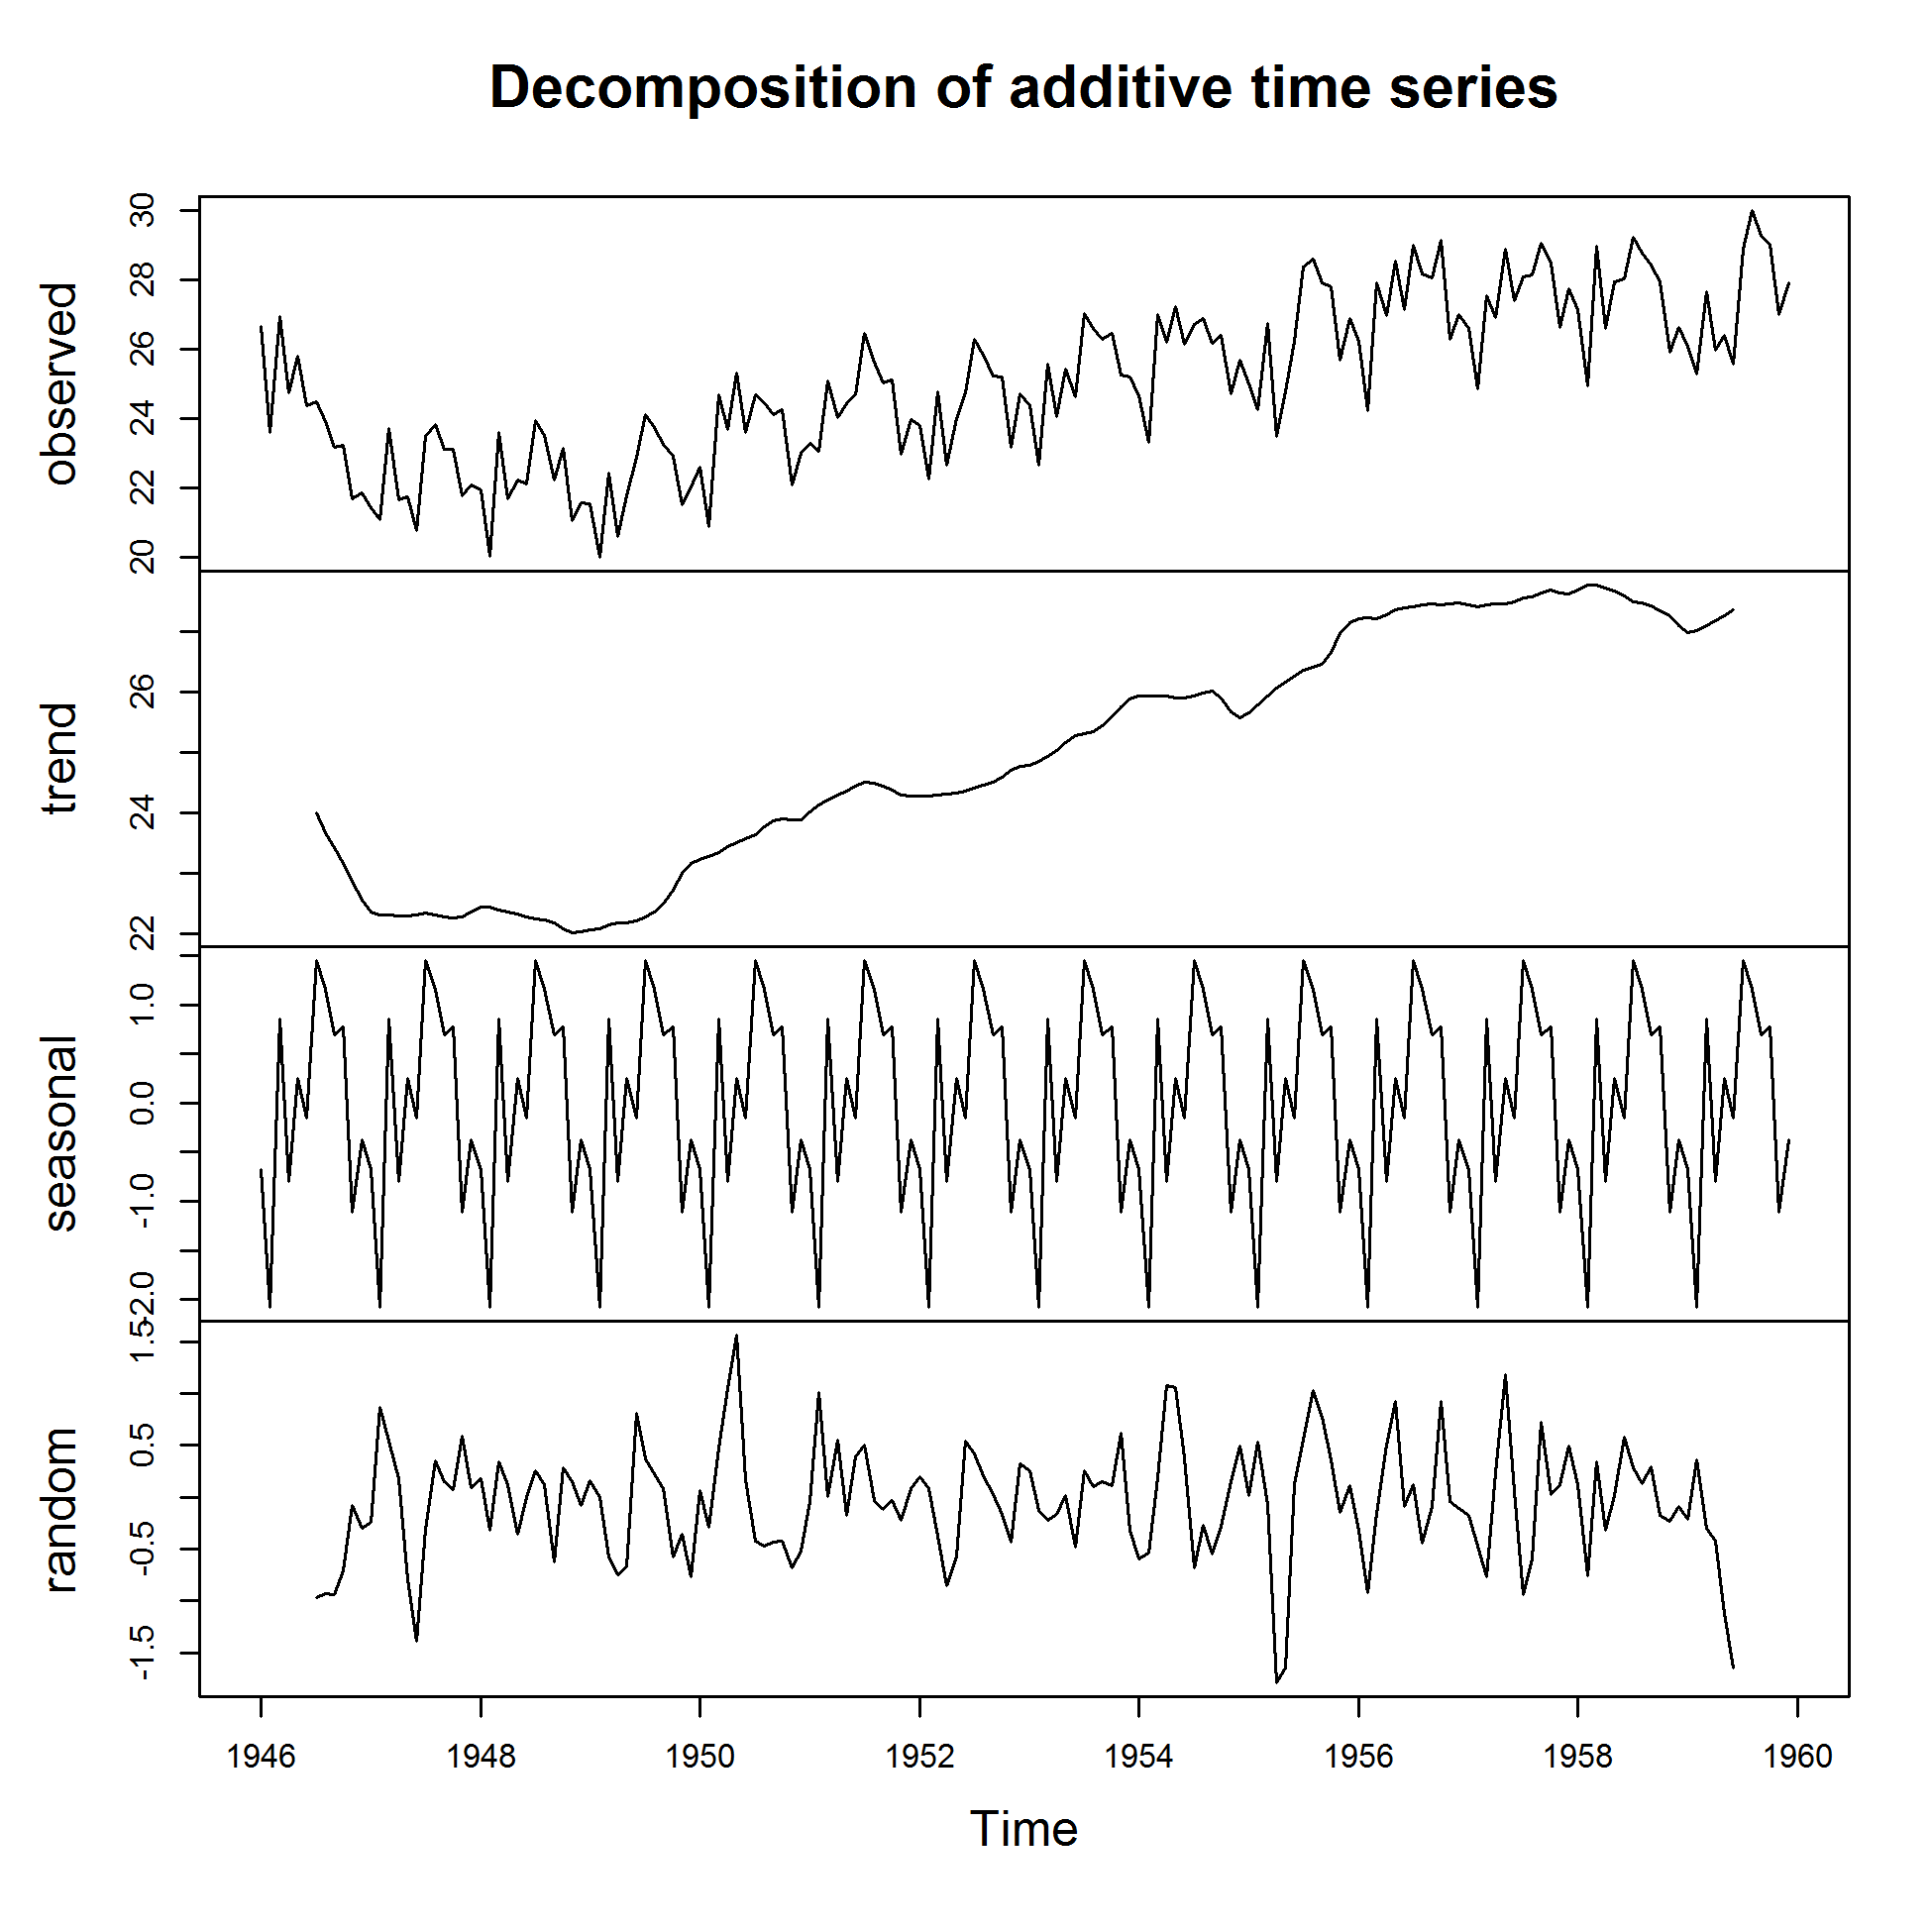
\includegraphics[width=0.8\textwidth]{time_series_components.png}
  \caption{Príklad dekompozície additívne časového radu~\cite{Madison2016}.}
  \label{fig-time-comp}
\end{figure}

\subsubsection{Zložky časových radov}
Pri predpovedaní časových radov ako napr. meraní odberu elektriky vznikajú
2 typy trendov. Prvým typom je trvalá alebo dočasná zmena spôsobená
ekonomickými alebo ekologickými faktormi. Druhým typom je sezónna zmena,
spôsobená zmenami ročných období a množstvom denného svetla. Môžeme ju pozorovať
na úrovni dňov, týždňov alebo rokov. Veličina, ktorú sa snažíme predpovedať
postupne mení svoje správanie a model sa tak stáva nepresným. Kvôli tomu je
nutné v každom modely rozdeľovať tieto typy tendencií, aby sme vedeli model
zmenám prispôsobiť~\cite{Grmanova2016}.

Vo všeobecnosti sú časové rady zložené zo 4 hlavných zložiek, ktoré môžeme
odlíšiť od pozorovaných dát. Jedná sa o trendovú, cyklickú, sezónnu
a reziduálnu zložku~\cite{Agrawal2013}.

\paragraph{Trendová zložka} predstavuje správanie časového radu v dlhodobom
časovom horizonte. Z tohto pohľadu má časový rad tendenciu klesať, rásť alebo
stagnovať. Príkladom môže byť nárast populácie či klesajúca
úmrtnosť~\cite{Agrawal2013}.

\paragraph{Cyklická zložka} je spôsobená zmenami, ktoré sa cyklicky opakujú.
Dĺžka periódy je 2 a viac rokov, čo zodpovedá strednodobému časovému horizontu.
Táto zložka je zastúpená najmä pri ekonomických časových radoch napríklad
podnikateľský cyklus pozostávajúci zo 4 fáz, ktoré sa stále
opakujú~\cite{Agrawal2013}.

\paragraph{Sezónna zložka} predstavuje kolísanie časových radov počas ročných
období. Dôležitými faktormi pri tom sú napr. klimatické podmienky, tradiície
 alebo počasie. Napríklad predaj zmrzliny sa v lete zvyšuje, ale počet
 predaných lyžiarskych súprav klesá~\cite{Agrawal2013}.

\paragraph{Reziduálna zložka} predstavuje veličinu, ktorá nemá žiadny
opakovateľný vzor a ani dlhodobý trend. V časových radoch má nepredvídateľný
vplyv na pozorovanú veličinu. V štatistike zatiaľ nie je definovaná metóda na
jej meranie. Označuje sa aj ako náhodná zložka alebo biely šum. Je spôspobená
nepredvídateľnými a nepravideľnými udalosťami~\cite{Agrawal2013}.

Vo všeobecnosti sa pre tieto 4 zložky používajú 2 rôzne modely. Je to
multiplikatívny model a aditívny model.
\begin{equation}
  \begin{split}
    Y(t) = T(t) \times S(t) \times C(t) \times I(t)
    \\
    Y(t) = T(t) + S(t) + C(t) + I(t)
  \end{split}
  \label{eq-ts-models}
\end{equation}
Vo vzorci~\ref{eq-ts-models} predstavuje $Y(t)$ meranie v čase $t$. Premenné
$T(t)$, $S(t)$, $C(t)$ a $I(t)$ sú zložkami trendu, sezónnosti,
cyklu a náhodnosti. Multiplikatívny model je založený na predpoklade, že časové
rady môžu byť na sebe závislé a môžu byť ovplyvňované medzi sebou, zatiaľ čo
aditívny model predpokladá nezávislosť zložiek~\cite{Agrawal2013}.

%-------------------------------------------------------------------------------
%   Analysis of prediction algorithms
%-------------------------------------------------------------------------------

\subsection{Analýza predičkných algoritmov}
Na základe množstva predikčných

%-------------------------------------------------------------------------------
%   Linear regression
%-------------------------------------------------------------------------------

\subsubsection{Lineárna regresia}
Najpoužívanejšia štatistická metóda, ktorá modeluje vzťah závislej premennej
a vysvetľujúcej premmennej. Závislú premmenu predstavuje veličina, ktorú sa
snažíme predpovedať, čo je v našom prípade spotreba elektriky. Vysvetľujúca
premenná v sebe zahŕňa rôzne faktory, ktoré ovplyvňujú závislú premennú.
Môžeme si pod tým predstaviť deň v týždni, počasie, tradície alebo rôzne
udalosti, ktoré majú vplyv na predpoveď.~\cite{KumarSingh2013, Mahalakshmi2016}.

Predpokladajme typický regresný problém. Dáta pozostávajúce z množiny \textit{n}
meraní majú formát $\left\{(x_1, f(x_1)), ..., (x_n, f(x_n))\right\}$.
Úlohou regresie je odvodiť funkciu $\hat{f}$ z dát, kde
\begin{equation}
  \hat{f} : X \to \mathbb{R} \text{, kde, } \hat{f}(x) = f(x), \forall x \in X,
  \label{eq-regresia}
\end{equation}
Funkcia $f$ vo vzorci~\ref{eq-regresia} reprezentuje reálnu neznámu
funkciu. Algoritmus použitý na odvodenie funkcie $\hat{f}$ sa nazýva
indukčný algoritmus. Funkcia $\hat{f}$ sa nazýva model alebo
prediktor. Obvykle je úlohou regresie minimalizovať odchýlku funkcie pre
štvorcovú chybu, konkrétne strednú štvorcovú chybu MSE~\cite{Mendes-Moreira2012}.

Keďže časový rad pozostáva z viacerých zložiek, môžeme ho zapísať ako funkciu
$L(t)$ definovanú ako
\begin{equation}
  L(t) = Ln(t) + \sum a_i x_i(t) + e(t)
  \label{eq-odber}
\end{equation}
Vo vzorci~\ref{eq-odber} funkcia $Ln(t)$ predstavuje odber elektriky v čase
$t$. Hodnota $a_i$ je odhadovaný pomaly meniaci sa koeficient. Faktory
$x_i(t)$ nezávisle vplývajú na spotrebu elektriky. Môže sa jednať napríklad
o počasie alebo zvyky ľudí. Komponent $e(t)$ je biely šum, ktorý má nulovú
strednú hodnotu a pevnú varianciu. Číslo $n$ je počet meraní, obvykle 24
alebo 168, v našom prípade 96 meraní počas jedného dňa~\cite{KumarSingh2013}.

\paragraph{Lineárna regresná analýza} je štatistická metóda používaná na
modelovanie vzťahov, ktoré môžu existovať medzi veličinami. Nachádza súvislosti
medzi závislou premennou a potenciálnymi vysvetľujúcimi premennými. Používame
pri tom vysvetľujúce premenné, ktoré môžu byť namerané súčasne so závislými
premennými alebo aj premenné z úplne iných zdrojov. Regresná analýza môže byť
tiež použitá na zlúčenie trendu a sezónných zložiek do modelu. Keď je raz model
vytvorený, môže byť použitý na zásah do spomínaných vzťahov alebo, v prípade
dostupnosti vysvetľujúcich premenných, na vytvorenie predikcie~\cite{Liu1992}.

\paragraph{Viacnásobná lineárna regresia} sa snaží modelovať vzťah medzi dvoma
alebo viacerými vysvetľujúcimi premennými a závislou premennou vhodnou
lineárnou rovnicou pre pozorované dáta. Výsledný model je vyjadrený ako funkcia
viacerých vysvetľujúcich premenných~\cite{Grmanova2016}.

Túto funkciu môžeme zapísať ako
\begin{equation}
  Y(t) = V_t a_t + e_t
  \label{eq-multi-regresia}
\end{equation}
Vo vzorci~\ref{eq-multi-regresia} $t$ označuje čas, kedy bolo meranie
uskutočnené. $Y(t)$ predstavuje celkový nameraný odber elektriky. Vektor $V_t$
reprezentuje hodnoty vysvetľujúcich premenných v čase merania. Vysvetľujúce
premenné môžu predstavovať meteorologické vplyvy, ekonomický nárast, ceny
elektriky či kruzy mien. Chybu modelu v čase $t$ zapíšeme
ako $e_t$~\cite{KumarSingh2013, Mahalakshmi2016}.

%-------------------------------------------------------------------------------
%   Stochastic models
%-------------------------------------------------------------------------------

\subsubsection{Stochastické modely}
Tieto metódy časových radov sú založené na predpoklade, že dáta majú vnútornú
štruktúru, ako napr. autokoreláciu, trend či sezónnu variáciu. Najprv sa
precízne zostaví vzor zodpovedajúci dostupným dátam a potom sa na jeho základe
predpovie budúca hodnota veličiny~\cite{KumarSingh2013}.

\paragraph{Autoregresný model} predpovedá budúcu hodnotu premmennej ako súčet
lineárnej kombinácie $p$ predchdzajúcich meraní, náhodnej chyby a konštanty.
V literatúre sa označuje ako AR (autoregressive model). Matematicky môžeme
autoregresný model zapisať ako
\begin{equation}
  y_t = c + \sum_{i=1}^{p} \varphi_i y_{t-i} + \varepsilon_t
  \label{eq-ar}
\end{equation}
Vo vzorci~\ref{eq-ar} hodnota $y_t$ predstavuje predpovedanú hodnotu
v čase $t$. Náhodnú chybu v čase $t$ zapíšeme ako $\varepsilon_t$. Hodnoty
$\varphi_i$ sú parametre modelu a $c$ je konštanta. Konštantou $p$ označujeme
rad modelu~\cite{Agrawal2013}.

\paragraph{Model kĺzavého priemeru} na rozdiel od autoregresného modelu používa
ako vysvetľujúce premenné chyby predchádzajúcich meraní a nie priamo hodnoty.
V literatúre sa označuje ako MA (moving average). Matematicky môžeme tento
vzťah zapísať ako
\begin{equation}
  y_t = \mu + \sum_{j=1}^{q} \Theta_j \varepsilon_{t-j} + \varepsilon_t
  \label{eq-ma}
\end{equation}
Vo vzorci~\ref{eq-ma} hodnota $y_t$ predstavuje strednú hodnotu
postupnosti meraní v čase $t$. Hodnoty $\Theta_j$ sú parametre modelu
a konštantou $q$ označujeme rad modelu. Vychádzame z predpokladu, že náhodná
zložka $\varepsilon_t$ je biely šum, čo je rovnomerne distribuovaná náhodná
premenná, ktorá má nulovú strednú hodnotu a konštantnú varianciu
$\sigma^2$~\cite{Agrawal2013}.

\paragraph{Autoregresívny model kĺzavého priemeru} reprezentuje súčasnú hodnotu
časového rádu linárne na základe jeho hodnôt a hodnôt bieleho šumu
v predchádzajúcich periódach. V literatúre sa označuje ako ARMA (autoregressive
moving average)~\cite{KumarSingh2013}.

Ide o kombináciu autoregresie (AR) a kĺzavého priemeru (MA), vhodnú pre
modelovanie jednorozmerných časových radov. Matematicky môžeme reprezentovať
tento model ako súčet predchádzajúcich modelov
\begin{equation}
  y_t = c + \varepsilon_t + \sum_{i=1}^{p} \varphi_i y_{t-i}  \sum_{j=1}^{q} \Theta_j \varepsilon_{t-j}
  \label{eq-arma}
\end{equation}
Rad modelu určuje $p$ a $q$~\cite{Agrawal2013}.

\paragraph{Autoregresívny integrovaný model kĺzavého priemeru} je
generalizáciou modelu ARMA. V literatúre sa označuje ako ARIMA (autoregressive
integrated moving average). Modely typu ARMA môžu byť použité iba na statické
časové rady. Mnoho časových radov v praxi vykazuje nestatické správanie a napr.
tie, ktoré obsahujú komponenty trendu a sezónnosti. Kvôli tomu bol navrhnutý
model ARIMA, ktorý je zahŕňa v sebe aj prípady nestatických časových radov.
Z nestatických časových radov sa vytvárajú statické pomocou konečného počtu
derivovaní dátových bodov. Vzniká tak matematický model, ktorý môžeme zapísať
ako
\begin{equation}
  \Big( 1 - \sum_{i=1}^{p} \varphi_i L^i \Big) (1-L)^d y_t = \Big( 1 + \sum_{j=1}^{q} \Theta_j L^j \Big) + \varepsilon_t
  \label{eq-arima}
\end{equation}
Vzorec~\ref{eq-arima} môžeme zapísať aj jednoduchšie a to
\begin{equation}
  \varphi(L) (1-L)^d y_t = \Theta(L) \varepsilon_t
  \label{eq-arima-short}
\end{equation}
Vo vzorci~\ref{eq-arima} predstavujú premenné $p$, $d$ a $q$ rad autoregresného
modelu, modelu kĺzavého priemeru a integrovaného modelu. Hodnota $d$ zodpovedá
stupňu derivovania, zvyčajne je rovná 1. V prípade, že $d=0$ dostaneme klasický
ARMA model. Rovnakým spôsobom vieme dostať modely AR a MA~\cite{Agrawal2013}.

%-------------------------------------------------------------------------------
%   Support vector regression
%-------------------------------------------------------------------------------

\subsubsection{Support vector regression}
Support Vector Machine a Support Vector Regression sú založené na štatistickej
teórií učenia, nazývanej aj VC teória, podľa svojich autorov, Vapnik
a Chervonenkisa~\cite{Sapankevych2009}.

Support Vector Machine je použité na množstvo úloh strojového učenia ako je
rozoznávanie vzorov, klasifikácia objektov a v prípade predikcií časových
radov to je regresná analýza. Support Vector Regression je postup, ktorého
funkcia je predpovedaná pomocou nameraných dát, ktorými je Support Vector
Machine postupne natrénované. Toto je odklon od tradičných predpovedí časových
radov, v zmysle že Support Vector Machine nepoužíva žiadny model, ale
predikciu riadia samotné dáta~\cite{Sapankevych2009}.

Táto predikčná metóda poskytuje malý počet voľných parametrov. Garantuje
konvergenciu k ideálnemu riešeniu a môže byť výpočtovo
efektívna~\cite{Sapankevych2009}.

%-------------------------------------------------------------------------------
%   Decision trees
%-------------------------------------------------------------------------------

\subsubsection{Rozhodovacie stromy}
Rozhodovacie stromy sú jednou z najrozšírenejších učiacich metód. Používajú sa
najmä na klasifikáciu, ale v súčasnosti sa využívajú aj na regresiu.
Rozhodovací strom je reprezentovaný ako množina uzlov a im prislúchajúcich
hrán. Uzly reprezentujú atribúty a výstupné hrany sú vždy označené konkrétnou
hodnotou pre atribút, z ktorého vychádzajú. Rozhodovanie začína v koreni stromu
a končí po dosiahnutí listového uzla. Pre riešenie jedného problému je možné
vytvoriť stromy s rôznym počtom a usporiadaním uzlov. Najlepším riešením je
strom s najmenším počtom rozhodovacích uzlov~\cite{Merz1998}.

\paragraph{Regresný rozhodovací strom}

%-------------------------------------------------------------------------------
%   Random forest
%-------------------------------------------------------------------------------

\subsubsection{Náhodné lesy}
Náhodné lesy sú kombináciou predpovedí stromov. Každý strom závisí od hodnoty
náhodného vektora s rovnakým rozdelením. Chyba lesu závisí od sily jednotlivých
strom a koreláciou medzi nimi. Náhodný les môžeme definovať ako klasifikátor
pozostávajúci z množiny stromov $\{h(x, \Theta_k), k=1, 2, ... \}$, kde
$\{\Theta_k\}$ sú nezávislé rovnomerne distribuované náhodné vektory a každý
strom sa podiela na hlasom na voľbe triedy vstupu $x$. S nárastom počtu stromov
hodnota $\{\Theta_k\}$ konverguje k určitému bodu. Tým je zabezpečené, že
náhodné lesy sa s pridávajúcim počtom stromov nepretrénujú ale veľkosť chyby sa
postupne ústáli. Pri výbere náhodného vektora sa snažíme pri zachovaní jeho
sily minimalizovať koreláciu, čím zvyšujeme presnosť celého
výpočtu~\cite{Breiman2001}.

Väčšinou sú náhodné lesy používané na klasifikačné problémy, avšak je možné ich
aplikovať aj na regresiu. Regresné náhodné lesy sú tvorené rastom stromov
závyslých na náhodnom vektore $\{\Theta\}$. Prediktor stromu $h(x, \Theta)$
nadobúda číselné hodnoty narozdiel od štíkov tried ako je to pri klasifikačných
problémoch. Predpokladáme trénovaciu množinu, ktorá je nezávislou distribúciou
náhodneho vektora $Y, X$. Potom môžeme strednú štvorcovú generalizačnú chybu
pre číselný prediktor $h$ matematicky zapísať ako
\begin{equation}
  E_{X, Y} (Y - h(X))^2
  \label{eq-random-error}
\end{equation}
Prediktor náhodného lesu je tvorený priemerom $k$ stromov, čo zapíšeme ako
$h(x, \Theta_k)$~\cite{Breiman2001}.

%-------------------------------------------------------------------------------
%   Neural networks
%-------------------------------------------------------------------------------

\subsubsection{Neurónové siete}
Neurónové siete sú inšpirované činnosťou mozgu a nervovej sústavy.

Neurónová sieť predstavuje orientovaný graf uzlov. Každý uzol počíta svoj
výstup na základe vstupov od susedných uzlov. Výpočet prebieha aplikovaním
funkcie, ktorá sa nazýva sigmoid, na vážený súčet vstupov. Uzol neurónovej
siete sa označuje ako neurón~\cite{Gruau1994}.

Je veľa typov neurónových sietí napríklad viacvrstvové perceptónové siete,
samoriadiace siete, siete s viacerými skrytými vrstvami atď. V každej skrytej
vrstve je množstvo neurónov. Hlavnou výhodou je, že väčšina sietí nepotrebuje
model. Na druhej strane, trénovanie obvykle zaberá veľa času. Výstupom siete
je lineárna rovnica váh prepojených so vstupom~\cite{KumarSingh2013}.

Najpoužívanejšou neurónovou sietou je viacvrstvový perceptón, ktorý pozostáva
z uzlov a im prislúchajúcim hranám. Uzly sú zoskupované do rôznych vrstiev.
Prvá vrstva je vstupná vrstva, kde počet $d$ označuje počet vstupných parametrov
vstupujúcich do siete. Táto vrstva je následne prepojená hranami so skrytou
vrstvou pozostávajúcou z $h$ uzlov. Tá je potom prepojená s výstupnou vrstvou
s $c$ uzlami. Kvôli tomu sa tieto siete zvyknú označovať aj ako dopredné
siete~\cite{Merz1998}.

Elementy skrytých a výstupných vrstiev sú umelé neuróny pozostávajúce z uzlov,
viacerých vstupujúcich a jednou výstpnou hranou. Funkciou neurónu je
transformovať lineárnu kombináciu vstupov pomocou nelineárnej aktivačnej
funkcie, čiže každú vstupnú hranu prenásobiť jej váhou a výsledok týchto súčinou
sčítať. Tak dostaneme pre neurón $j$ vzorec~\ref{eq-linear-combination}
opisujúci lineárnu kombináciu vstupov $a_j$
\begin{equation}
  a_j = \sum_{i=1}^{d} w_{ji} x_i
  \label{eq-linear-combination}
\end{equation}
Príčom váha $w_{ji}$ označuje váhu medzi neurónom $i$ na vstupnej vrstve
a neurónom $j$ na skrytej vrstve~\cite{Merz1998}.

Aktivovanie neurónu $j$ závisí od jeho aktivačnej funkcie $g(a_j)$. Jednu
z najpoužívanejších aktivačných funkcií, logistickú sigmoidnú funkciu, môžeme
matematicky zapísať ako
\begin{equation}
  g(a) \equiv \frac{1}{1 + exp(-a)}
  \label{eq-sigmoid-function}
\end{equation}
Je zrejmé, že funkcia zo vzoraca~\ref{eq-sigmoid-function} vracia hodnoty
v rozmedzí $(0,1)$~\cite{Merz1998}.

%-------------------------------------------------------------------------------
%   Ensemble learning
%-------------------------------------------------------------------------------

\subsubsection{Učenie súborov klasifikátorov}
Používa sa na jednodňovú predikciu. Ak \textit{h} je počet meraní, ktoré sú
denne dostupné, v deň \textit{t} sa vykoná \textit{h} predikcií podľa váženého
priemeru \textit{m} modelmi. Nasledujúci deň sa vypočíta chyba predpovede,
na základe ktorej sa znova prepočítajú váhy a každý model sa
aktualizuje\cite{Grmanova2016}.

Učenie súborov klasifikátorov môžeme rozdeliť na homogénne a heterogénne učenie.

\paragraph{Homogénne učenie súborov klasifikátorov}
Pozostáva z modelov rovnakého typu, ktoré sa učia na rôznych podmnožinách
datasetu.
\paragraph{Heterogénne učenie súborov klasifikátorov}
Aplikuje rôzne typy modelov nad rovnakými dátovými množinami\cite{Grmanova2016}.

%-------------------------------------------------------------------------------
%   Exponential smoothing
%-------------------------------------------------------------------------------

\subsubsection{Exponencionálne vyrovnávanie}

Táto metóda, tak ako vyššie popísané metódy, najprv na základe dát
z predchádzajúcich meraní vytvorí model. Ten sa v ďalej použíje na
redpovedanie budúcich dát. Tento vzťah môžeme matematicky zapísať ako
\begin{equation}
  y(t) = \beta(t)^T f(t) + \varepsilon(t)
  \label{eq-expo}
\end{equation}
Vo vzorci \ref{eq-expo} sa opäť nachádza biely šum $\varepsilon(t)$. Hodnota
$\beta(t)$ predstavuje \textbf{coefficient vector} a $f(t)$
\textbf{fitting function}~\cite{Mahalakshmi2016}.

Jednou z predikčných metód časových radov, ktorá používa exponencionálne
vyrovnávanie je aj Wintersova metóda. Pri sezónnych dátach sú použité 3
vyrovnávacie parametre a to trend, sezónosť a stacionárnosť. Analýza
a predpoveď priamym aplikovaním Wintersovej metódy môže byť náročné, keďže
dátové množiny väčšinou obsahujú \textbf{riedke pozorovania (sparse values)}.
Tento problém môžeme vyriešiť kombináciou ostatných metód, ako je napr.
autoregresívny model či spektrálna analýza, s exponencionálnym
vyrovnávaním~\cite{Mahalakshmi2016}.



%-------------------------------------------------------------------------------
%   Naive methods
%-------------------------------------------------------------------------------

\subsubsection{Naivné metódy}
Predpovede sú vytvárané pomocou posledných hodnôt alebo ich priemerov.

\paragraph{Seasonal naïve method}
Poslednú nameranú hodnotu použijeme ako predpoveď pre nasledujúce obdobie. Ak
sú naše dáta vysoko závisle od ročného obdobia, je lepšie použiť na predpoveď
hodnotu z rovnakého obdobia, napr. z minulého roka~\cite{Grmanova2016}.

\paragraph{Naïve average long-term method}
Predpokladá, že dáta obsahujú vzory, ktoré nie sú závislé od ročných období.
Kvôli tomu sú časové rady lokálne stabilné s pomaly meniacim sa priemerom.
Hodnotu, ktorú použijeme ako predpoveď je iba priemorom viacerých posledných
hodnôt~\cite{Grmanova2016}.

\paragraph{Naïve In median long-term method}
Táto metóda je alternativou k predchádzajúcej metóde. Keďže priemerom nedokáže
model dostatočne rýchlo reagovať na rapídne výkyvy a abnormality, lepšie
výsledky dosiahneme nahradením priemeru za median posledných \textit{n}
meraní~\cite{Grmanova2016}.

%-------------------------------------------------------------------------------
%   Analysis of optimizing algorithms
%-------------------------------------------------------------------------------

\subsection{Analýza optimalizačných algoritmov}

% definicia optimalizacnz algoritmov
% preco optimalizacne algoritmy a nie hocco ine


%-------------------------------------------------------------------------------
%   Genetic algorithms
%-------------------------------------------------------------------------------

\subsubsection{Genetické algoritmy}
Jedná sa o bilogicky inšpirované algoritmy patriace do triedy
evolučných algoritmov. Genetické algoritmy sú stochastické optimalizačné
algortimy s \textbf{global search potential}. Od tradičných algoritmov sa líšia
hlavne v počte riešení, ktoré sú kandidátmi na najlepšie riešenie. Tradičné
vyhľadávacie algoritmy prehľadávajú dôkladne iba jedno riešenie, zatiaľ čo
genetické algoritmy hlbšie spracujú viacero kandidátou naraz. Každý kandidát na
optimálne riešenie problému je reprezentovaný dátovou štruktúrou, ktorú
označujeme pojmom jedinec. Súbor jedincov tvorí populáciu. Začiatok procesu
začína náhodnými riešeniami populácie, ktorý sa postupne
vylepšuje~\cite{Chavan2015}.

Pri genetických algoritmoch sa zavádzajú pojmy ako chromozón, fitness funkcia,
kríženie, elitárstvo, operátor reprodukcie či mutácie~\cite{Chavan2015}.

Vytvorenie novej generácie prebieha pomocou genetického operátora,
a to selekciou, krížením a mutáciou. Proces selekcie vyberie kvalitnejšie
chromozóny, ktoré prežijú a vyskytnú sa tak aj v ďalšej generácii. Tiež sa
vyberajú nekvalitné chromozóny, ktoré zahynú a nebudú ďalej brané do
úvahy~\cite{Simonova2007}.

Princíp fungovania genetických algoritmov možno znázorniť v nasledujúcom
pseudokóde~\cite{Chavan2015}
\begin{algorithm}
  \caption{Pseudokód genetického algoritmu}
  \begin{algorithmic}[1]
    \State Náhodne inicializovanie jedincov Inicializácia
    \State Vyhodnotenie fitness funkcie pre každého jedinca \label{ga-fitness}
    \State Výber jedincov pre ďalšiu populáciu na základe fitnesss funkcie \label{ga-selection}
    \State Kríženie jedincov \label{ga-crossing}
    \State Mutovanie jedincov \label{ga-mutation}
    \State Kontrola či nebolo nájdené žiadané optimálne riešenie \label{ga-condition}
    \State Ukončenie ak sa našlo takéto riešenie, inak opakovanie krokov \ref{ga-fitness} až \ref{ga-condition}
    \State Koniec
  \end{algorithmic}
\end{algorithm}

Veľkou výhodou genetických algoritmov je, že mutácia predchádza skĺznutiu do
lokálnych miním a rekombinácia chromozónov vedie k rýchlemu približovaniu
sa k optimálnemu riešeniu. Napriek týmto výhodám, majú genetické algoritmy aj
niekoľko nevýhod~\cite{Deolekar2016}.
\begin{itemize}
  \item Reprezentovanie kandidátov je príliš obmedzujúce
  \item Mutácia a kríženie sú v súčasnosti aplikovateľné iba na chromozóny
        reprezentované bitovým reťazcvom alebo číslami
  \item Definovanie fitness funkcie je často netriviálnou záležitosťou
        a jej generalizácia je náročná
\end{itemize}

\paragraph{Chromozón} je pomenovanie pre jedinca. V literatúre sa tiež zvykne
používať označenie kandidát~\cite{Arun2016}.

\paragraph{Fitness funkcia} je funkcia určujúca efektívnosť chromozónu, pre
ktoré je vypočítaná fitness funkcia. Pri hľadaní optimálneho riešenia sa
porovnáva hodnota fitness funkcie aktuálneho riešenie s hodnotou funkcie
cieľového riešenia~\cite{Chavan2015, Simonova2007}.

\paragraph{Operátor reprodukcie} je obvykle prvý operátor, ktorý sa uplatní na
populáciu. Operátor náhodne vyberie reťazce z dvoch chromozónov na
párenie~\cite{Chavan2015}.

\paragraph{Kríženie} je operátor \textbf{recombination}. Kríženie vykonáva
výmenu blokov chromozónov. Z druhého chromozónu je vybraný reťazec náhodnej
veľkosti, ktorý sa vymení s rovnako dlhým reťazcom z prvého
chromozónu~\cite{Chavan2015}.

Vzniká problém ako, čo najvhodnejšie, určiť bod kríženia a vybrať tak
najkvalitnejšie bloky chromozónu. Kvôli tomu je potrebné definovať nový element
nazývaný väzba, označovaný ako $d_i$
\begin{equation}
  d_i = \frac{a_i + a_{i+1}}{2}
  \label{eq-crossing}
\end{equation}
Za predpokladu, že chromozón reprezentujeme ako maticu veľkosti $1 \times N$,
potom väzbu definovanú vzorcom \ref{eq-crossing} môžeme rezprezntovať ako
maticu $1 \times (N-1)$. Vypočítaním priemeru susedných hodnôt aj pre cieľovú
maticu a nájdením priemeru matice, určíme body kríženia. Chromozón rozdelíme na
miestach, kde je väzba, čo najmenšia~\cite{Simonova2007}.

\paragraph{Elitárstvo} je to proces pridávania chromozónov s najlepšou hodnotou
funkcie fitness priamo do ďalšej populácie. Zaisťuje to, že najlepšie riešenie
budúcej generácie bude vždy lepšie alebo pri najhoršom rovnaké ako najlepšie
riešenie predchádzajúcej generácie~\cite{Deolekar2016}.

\paragraph{Operátor mutácie} sa vykoná po vykonaní operátora reprodukcie.
Mutácia chromozónu väčšinou predstavuje operáciu, ktorá s nízkou
pravdepodobnosťou invertuje jeden bit v chromozóne~\cite{Chavan2015}.

%-------------------------------------------------------------------------------
%   Grey wolf optimizer
%-------------------------------------------------------------------------------

\subsubsection{Grey wolf optimizer}
Algoritmus je založený na správaní vlka dravého, ktorý je na vrchole
potravinového reťazca a preferuje život vo svorke. Lov pozostáva zo stopovania,
naháňania, približovania sa, obkľúčenia, obťažovaním koristi, pokiaľ neprestane
utekať a útokom na korisť. Vlkov vo svorke možno
rozdeliť do niekoľko skupín~\cite{Seeley1991}.

\paragraph{Alfa vlky} sú vodcami svorky. Ich úlohou je robiť rozhodnutia
ohľadom lovu, miesta na spanie či času zobudenia. Tieto príkazy diktujú svorke,
avšak bolo pozorované aj demokratické správanie, kedy alfa vlky nasledovali
ostatné vlky zo svorky. Pri stretnutí svorky dávajú všetky vlky najavo uznanie
alfa vlkov stiahnutým chvostom. Zaujímavosťou je, že vodcom svorky nemusí byť
najsilnejší jedinec, ale môže to byť aj jedinec najlepší v organizovaní
svorky~\cite{Seeley1991}.

\paragraph{Beta vlky} sp druhým stupňom v hierarchii vlčej svorky, podriadené
alfa vlkom, ktorým pomáhajú v rozhodovaní a organizácií svorky. Sú najlepšími
kandidátmi na alfa vlkov v prípade úmrtia alebo zostarnutia alfa vlkov. Mali by
rešpektovať alfa vlky a organizovať nižšie postavené vlky. Hrajú rolu radcu
a ďalej distribujú príkazy a vracajú sa s odozvou na ne~\cite{Seeley1991}.

\paragraph{Delta vlky} inak nazývané aj podriadené vlky zastupujú vo svorke
úlohy prieskumníkov, strážcov, starejších, lovcov či opatrovateľov.
Prieskumníci hliadkujú hranice teritória a varujú svorku v prípade akéhokoľvek
nebezpečia. Strážcovia zabezpečujú bežpečie svorky. Starejší sú skúsenými
vlkmi, ktorí boli alfa alebo beta vlkmi. Lovci pomáhajú alfa a beta vlkom pri
love a poskytujú svorke jedlo. Opatrovatelia sa starajú o slabé, choré alebo
zranené vlky~\cite{Seeley1991}.

\paragraph{Omega vlky} majú najnižšiu hodnosť vo svorke. Hrajú rolu obetných
baránkov, ktoré sa podrobia ostatným vlkom. Jedia úplne posledné. Aj keď sa
možno javí ich postavenie vo svorke zbytočné, boli pozorované prípady, kedy
ich strata spôsobila vo svorke nedorozumenia. Tiež slúžia na zbavenie sa
frustrácie ostatných vlkov, čím prispievajú k spokojnosti celej
svorky~\cite{Seeley1991}.

\paragraph{Spoločenská hierarchia} reprezentovaná matematickým modelom,
označuje najvhodnejšie riešenie ako alfa, druhé a tretie najvhodnejšie ako beta
resp. delta. Riešenia ostatných kandidátov označujeme ako omega. Algoritmus
optimalizácie (v prírode lovu) je vedený alfa, beta a delta kandidátmi, ktorí
sú nasledovaní kandidátmi omega~\cite{Seeley1991}.

\paragraph{Obkľúčenie koristi} môžeme matematicky reprezentovať ako
\begin{equation}
  \begin{split}
    \vec{D} = | \vec{C} \cdot \vec{X_p}(t) \vec{X}(t) |
    \\
    \vec{X}(t+1) = \vec{X_p}(t) - \vec{A} \cdot \vec{D}
  \end{split}
  \label{eq-prey-main}
\end{equation}
Aktuálnu iteráciu vo vzorci~\ref{eq-prey-main} zapíšeme ako $t$, vektor
$\vec{X_p}$ predstavuje vektor polohy koristi a $\vec{X}$ je vektor polohy
vlka. Vektory $\vec{A}$ a $\vec{C}$ sú koeficienty, ktoré zapíšeme ako
\begin{equation}
  \begin{split}
    \vec{A} = 2\vec{a} \cdot \vec{r_1} - \vec{a}
    \\
    \vec{C} = 2 \cdot \vec{r_2}
  \end{split}
  \label{eq-prey-minor}
\end{equation}
Vo vzorci~\ref{eq-prey-minor} premenná $\vec{a}$ sa počas výpočtu lineárne
znižuje od 2 po 0. Vektory $\vec{r_1}$ a $\vec{r_2}$ sú náhodnými vektormi
v rozsahu [0, 1]. Vlk môže svoju pozíciu $(X, Y)$ aktualizovať v závislosti od
pozície koristi $(X^*, Y^*)$. Obrázok \ref{fig-wolf-pos} ilustruje možné
aktualizované pozície, ktoré môže najlepší agent dosiahnuť. Tieto pozície
získame aplikovaním vzorcov~\ref{eq-prey-main}~\cite{Seeley1991}.

\begin{figure}[ht]
  \centering
  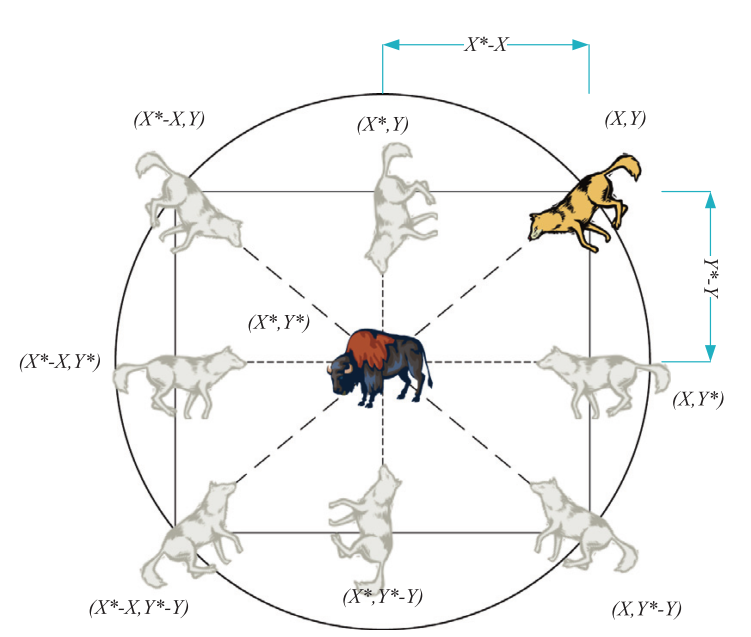
\includegraphics[width=0.8\textwidth]{wolf_vector_positions.png}
  \caption{Príklad možného umiestnenia vlka v dvojrozmernom priestore na základe polohy koristi.}
  \label{fig-wolf-pos}
\end{figure}

%-------------------------------------------------------------------------------
%   Artifical bee colony
%-------------------------------------------------------------------------------

\subsubsection{Umelá kolónia včiel}
V literatúre označovaný ako ABC algoritmus (Artifical bee colony) je pomerne
nový medzi rojovými algoritmami. Princíp je založený na biologickom procese,
správaní medonosných včiel pri hľadaní potravy. Hlavný mechanizmus ktorým včely
optimalizujú množstvo procesov je tzv. včelí tanec (\textbf{waggle dance}),
ktorým včely lokalizujú zdroje potravy a nachádzajú ďalšie~\cite{Chavan2015}.

Každá včela na pracujúca v roji sa spolupodiela na tvorbe celého systému na
globálnej úrovni. Správanie systému je určené lokálnym správaním, kde spolupráca
a zladenie jedincov vedie k štruktúrovanému kolaboračnému systému~\cite{Chavan2015}.

Algoritmus funguje na princípe, že včely nájdu najviac výnosný zdroj
s použitím, čo najmenšej energie. \textbf{Foragers} (zrejme robotnice hľadajúce zdroj jedla) uvažujú
presúvanie sa medzi zdrojmi nektárov na základe kvality alebo zisku zdroju.
Algoritmus poskytuje samo-manažovateľné a samo-organizované riešenie, vo svojej
podstate decentralizované, pre daný problém~\cite{Buhussain2016}.

%-------------------------------------------------------------------------------
%   Ant colony optimization
%-------------------------------------------------------------------------------

\subsubsection{Kolónia mravcov}
Pri tomto algoritme, mravce tiež opúšťajú mravenisko, kvôli hľadaniu zdrojov
potravy náhodne. Potom vyhodnotia kvalitu zdroja potravy a donesú ho naspäť do
mraveniska. Zanechávajú pri tom na zemi chemické stopy. Sila týchto stôp závisí
od kvality nájdeného zdroja potravy. Mnoho výskumov využíva tento algoritmus na
riešenie NP problémov, ako napríklad problém obchodných cestujúcich,
vyfarbovanie grafov, smerovnaie áut alebo plánovacie problémy. Používa sa aj pri
\textbf{cloud computing} na nájdenie optimálneho riešenia pri plánovaní úloh
pre virtuálne servery~\cite{Buhussain2016}.

Keď mravce hľadajú potravu prvý krát, hľadajú náhodne až kým nenájdu zdroj
potravy. Zanechávajú pri tom za sebou chemickú stopu nazývanú feromón, ktorá
tak vedie k zdroju. Tá následne priťahuje ostatné mravce k tomuto zdroju
potravy. Tento proces pokračuje pokiaľ mravce nenájdu najkratšiu cestu vedúcu
ku konkrétnemu zdroju potravy. Najkratšia cesta je určená naakumulovaným
množstvom feromónov na ceste k zdroju potravy~\cite{Buhussain2016}.

%-------------------------------------------------------------------------------
%   Measurement of prediction accuracy
%-------------------------------------------------------------------------------

\subsection{Meranie presnosti predpovedi}
Pre vyhodnotenie efektívnosti a presnosti modelov je potrebné merať ich
vlastnosti tak, aby sme ich vedeli medzi sebou porovnáva. V nasledujúcich
spôsoboch merania sú použité pojmy ako aktuálna hodnota $y_t$, predpovedaná
hodnota $f_t$ alebo chyba predpovede $e_t$ definovaná ako $e_t = y_t - f_t$.
Veľkosť testovacej množiny budeme označovať ako $n$~\cite{Agrawal2013}.

\subsubsection{Stredná chyba predpovede}
V literatúre označovaná ako MFE (mean forecast error). Matematickú funkciu
zapísať ako
\begin{equation}
  MFE = \frac{1}{n} \sum_{t=1}^{n} e_t
  \label{eq-mfe}
\end{equation}
Týmto spôsobom meriame priemernú odchýlku predpovedanej hodnoty od aktuálnej.
Zistíme tak smer chyby. Nevýhodou je, že kladné a záporné chyby sa vynulujú
a potom nie je možné zistiť presnú hodnotu chyby. Pri namerani extrémnych chýb,
nie sú nijak špeciálne penalizované. Taktiež hodnota chyby závisí od škály
meraní a môže byť ovplyvnená aj transformáciami dát. Dobré predpovede majú
hodnotu blízku 0~\cite{Agrawal2013}.

\subsubsection{Stredná absolútna chyba}
V literatúre označovaná ako MAE (mean absolute error). Patrí k jedným
z najpoužívanejších. Funkciu môžeme zapísať ako
\begin{equation}
  MAE = \frac{1}{n} \sum_{t=1}^{n} |e_t|
  \label{eq-mae}
\end{equation}
Týmto spôsobom meriame priemernú absolútnu odchýlku predpovedanej hodnoty od
aktuálnej. Zistíme tak celkový rozsah chyby, ktorá nastala počas predpovede.
Narozdiel od merania chyby pomocou vzorca~\ref{eq-mfe} sa kladné a záporné
chyby nevynulujú, no ani napriek tomu nevieme určiť celkový smer chyby.
Na druhej strane tiež nenastáva žiadna penalizácia pri extrémnych chybách,
hodnota chyby závisí od škály meraní, môže byť ovplynená transformáciami dát
a dobré predpovede majú hodnotu čo
najbližšiu 0~\cite{Agrawal2013, Gutierrez2015}.

\subsubsection{Stredná percentuálna chyba}
V označovaná ako MPE (mean percentage error). Matematciky môžeme túto funkciu
zapísať ako
\begin{equation}
  MPE = \frac{1}{n} \sum_{t=1}^{n} \frac{e_t}{y_t} \times 100
  \label{eq-mpe}
\end{equation}
Vlastnosti sú veľmi podobné ako pri MAPE v časti \ref{mape}. Chyba nám
poskytuje prehľad o priemernej chybe, ktorá sa vyskytla počas predpovede.
Naviac, oproti MAPE, získame prehľad o smere chyby, čo má však za následok, že
opačné znamienka sa vynulujú. O modely, ktorého chyba MPE sa blíži k 0
nemôžeme s určitosťou tvrdiť, že funguje správne~\cite{Agrawal2013}.

\subsubsection{Stredná aboslútna percentuálna chyba}
\label{mape}
V literatúre označovaná ako MAPE (mean absolute percentage error). Vzorec,
ktorým ju zapíšeme bude veľmi podobný vzorcu \ref{eq-mpe}
\begin{equation}
  MAPE = \frac{1}{n} \sum_{t=1}^{n} \Big|\frac{e_t}{y_t}\Big| \times 100
  \label{eq-mape}
\end{equation}
Pomocou tohto merania chyby získavame percentuálny prehľad o priemernej
absolútnej chybe, ktorá sa vyskytla počas predpovedi. Veľkosť chyby nezávisí od
škály merania, ale je závislá od transformácií dát. Tiež nie je možné zistiť
smer chyby a ani nenastáva žiadna penalizácia pri extrémnych
chybách~\cite{Agrawal2013}.

\subsubsection{Stredná štvorcová chyba}
V literatúre označovaná ako MSE (mean squarred error). Vzorcom ju zapíšeme ako
\begin{equation}
  MSE = \frac{1}{n} \sum_{t=1}^{n} e_t^2
  \label{eq-mse}
\end{equation}
Chyba meria priemernú štvorcovú odchýlku predpovedanej hodnoty. Opačné
znamienka sa neovplyvňujú. Neposkytuje nám pohľad na smer chyby. Zabezpečuje
penalizáciu extrémnych chýb. Zdôrazňuje fakt, že celková chyba je viac
ovplyvnená jednotlivými veľkými chybami ako viacerými malými. Nevýhodou je, že
chyba je veľmi citlivá na zmenu škály alebo transformáciu
dát~\cite{Agrawal2013}.

\subsubsection{Symetrická stredná absolútna percentuálna chyba}
V literatúre označovaná ako SMAPE

%-------------------------------------------------------------------------------
%   Chapter 3 - Analysis evaluation
%-------------------------------------------------------------------------------

\newpage
\section{Zhodnotenie analýzy}

%-------------------------------------------------------------------------------
%   Chapter 4 - Specification
%-------------------------------------------------------------------------------

\newpage
\section{Špecifikácia požiadaviek}

%-------------------------------------------------------------------------------
%   Chapter 5 -   Analysis evaluation
%-------------------------------------------------------------------------------

\newpage
\section{Návrh riešenia}

%-------------------------------------------------------------------------------
%   Chapter 6 - Implementation
%-------------------------------------------------------------------------------

\newpage
\section{Implementácia}

%-------------------------------------------------------------------------------
%   Chapter 7 - Evaluation
%-------------------------------------------------------------------------------

\newpage
\section{Zhodnotenie}

%-------------------------------------------------------------------------------
%   Chapter 8 - Technical documentation
%-------------------------------------------------------------------------------

\newpage
\section{Záver}

\newpage
\section{Technická dokumentácia}

%-------------------------------------------------------------------------------
%   Bibliography
%-------------------------------------------------------------------------------

\newpage
\addcontentsline{toc}{section}{Literatúra}
\bibliographystyle{iso-690/czechiso}
\bibliography{bibliography}

\end{document}

% \paragraph{Autoregressive model}
% môže modelovať profil záťaže za predpokladu, že zátaž je lineárnou kombináciou
% predchádzajúcich záťaží\cite{KumarSingh2013}.

% \paragraph{Support Vector Machine based Techniques}
% je metóda analyzujúca dáta a rozpoznávajúca vzory, používaná na roztriedenie
% a regresnú analýzu, kombinuje zovšeobecnené riadenie
% s technikou ??????\cite{KumarSingh2013}.
%
% \paragraph{Support Vector Machine}
% je ML algoritmus používaný ako na klasifikáciu tak na regresiu
% support vector sú koordináty jednotlivých meraní napr. muž a žena a ich merané veličny reprezentované na osy, ktoré sú hraničnými elementami rôznych skupín
% maximalizuje rozmädzie medzi support vektormi jednej kategórie a support vektormi druhej kategórie, rozhodovacia funkcia je definovaná podmnožinou testovacej vzorky (jednotlivé supprot vektory)
% v 2D sú kategórie oddelené čiarou vo viacrozmerných dimenziách rovinou
%
% \paragraph{Incremental SVM}
% základom je pridávanie % http://www.jmlr.org/papers/volume7/laskov06a/laskov06a.pdf
% nový bod má najskôr pridelenú váhu 0, ak toto pridelenie nie je optimálnym riešením, teda bod sa môže stať support vectorom,
% váhy ostatných vektorov a rozhodovací prah musia byť aktualizované kvôli získaniu optimálneho riešenia nad novou množinou support vektorov
%
% \paragraph{Linear SVM}
% linárna kombinácia elementov (features, črty) značí, že sa jedná aj o lineárny klasifikátor  % http://stackoverflow.com/questions/6160495/support-vector-machines-a-simple-explanation
% napr ak (w1 * x1 + w2 * x2) > C potom element patrí do skupiny A, hodnotami x1 a x2 je element definovaný, tak ako je bod definovaný x a y súradnicou
% w je váha a C rozhodovacií prah, čiže ak nejaký ohodnotený element neprekročí hranicu spadá do jednej skupiny, ak prekročí spadá do druhej
%
% \paragraph{Concept drift}
% je správanie premennej, ktorú sa snažím predikovať sa môže časom meniť,
% čím sa postupne stáva model menej a menej presný\cite{Grmanova2016}.
%
% \paragraph{Online algorithm}
% spracováva vstup sériovo kúsok po kúsku, vstupné dáta nie sú dostupné na začiatku výpočtu % http://stackoverflow.com/questions/11496013/what-is-the-difference-between-an-on-line-and-off-line-algorithm
% musí spracovať vstup v jednej iterácií bez žiadnej podrobnej znalosti budúcich vstupov % https://xlinux.nist.gov/dads/HTML/online.html
% viac dát, časové obmedzenia, môže sa časom meniť % http://stats.stackexchange.com/questions/897/online-vs-offline-learning
%
% \paragraph{Offline algorithm}
% rieši problém od začiatku so všetkými vstupnými dátami % http://stackoverflow.com/questions/11496013/what-is-the-difference-between-an-on-line-and-off-line-algorithm
% vopred je daná celá séria vstupov % https://xlinux.nist.gov/dads/HTML/offline.html

% \paragraph{Kernel trick}
% problém nie je lineárne separovateľný, originálny nelineárny priestor % http://stats.stackexchange.com/questions/3947/help-me-understand-support-vector-machines
% je premietnutý do viacrozmerného priesotru pomocou nejakej nelineárnej transofrmácia s očakávaním, že to problém už bude riešiteľný
%
% \paragraph{Extreme learning machine}
% je novovznikajúca technika učenia poskytujúca efektívne % http://cherup.yonsei.ac.kr/files/Paper/2013_IEEE%20Intelligent%20Systems%20-%20Off%20line%20version_A%20System%20for%20Signature%20Verification%20Based%20on%20Horizontal%20and%20Vertical%20Components%20in%20Hand%20Gestures.pdf
% a zjednotené riešenie na všeobecné dopredné siete ako
% neurónové siete, RBF siete alebo kernelové učenie

% Časový rád je súbor meraní presne definovaných veličín získavaných opakovanými
% meraniami. Dáta zbierané zriedkavo alebo jednorázovo nepovažujeme za časový rád.
% Pozorované časové rády možno rozložiť na 3 zložky a to trendovú, sezónnu
% a nepravidelnú\cite{AustralianBureau}.

% Trendová zložka predstavuje smer veličiny v dlhodobom horizonte a máva klesajúci
% alebo stúpajúci charakter. Na druhej strane, sezónna zložka má cyklický
% charakter a dĺžka cyklu sa viaže napr. ku dňu, týždnu či roku. Nepravidelná
% zložka reprezentuje náhodné zmeny v prostredí, ktoré nie sú relevantné pre
% predpoveď časových rádov. Pri trénovaní modelu sa ich snažíme odfiltrovať
% optimálnou mierou natrénovania modelu.

% Pri predpovedaní časových radov ako napr. meraní odberu elektriky vznikajú 2 typy tvz. Concept drift.
% \textbf{Concept drift} je zmena správania veličiny, ktorú sa snažíme
% predpovedať. Model sa tak stáva postupne nepresný a je potrebné aby sa tejto
% zmene prispôsobil. Prvým typom je trvalá alebo dočasná zmena spôsobená
% ekonomickými alebo ekologickými faktormi. Druhým typom je sezónna zmena,
% spôsobená zmenami ročných období a množstvom denného svetla. Sezónnu zmenu
% môžeme pozorovať na úrovni dní, týždňov alebo rokov. Kvôli tomu je nutné
% v každom modely rozdeľovať tieto 2 typy concept drift\cite{Grmanova2016}.

% \subsection{Reziduálna zložka}
% Ostáva v časovom rade po odstránení trendovej, cyklickej a sezónnej zložky.
% Je tvorená náhodnými pohybmi v priebehu časového radu. Tiež pokrýva chyby
% v meraní. Obvykle sa predpokladá, že reziduálna zložka je biely šum, teda
% nekorelované náhodné veličny s nulovou strednou hodnotou\cite{http://www.math.sk/mpm/otazka_30.pdf}.

% ε-insensitive loss function defined
% \[
%     L_{\varepsilon}(y, f(x, w)) =
%     \begin{cases}
%       0 \text{ ak } |y - f(x, w)| \leq \varepsilon \\
%       |y - f(x, w)| - \varepsilon \text{ inak } \\
%     \end{cases}
% \]

% \begin{equation}
%   fitness = \delta + P
%   \label{eq-fitness}
% \end{equation}
% Faktor $\delta$ predstavuje rozdieľnosť výrazu aktuálneho chromozónu od
% cieľového chromozónu \cite{Simonova2007}

% \paragraph{Logistický regresný model}
% Nelineárna diskriminantná štatistická metóda. V \textbf{binary response} modely
% os $y$ zvyčajne reprezentuje individuálnu alebo experimentálnu jednotku. $Y$ môže
% nadobúdať hodnoty 0 alebo 1 pre situácie kedy udalosť nastane alebo nenastane.
% Os $x$ reprezentuje vysvetľujúcu veličinu ako vektor, ktorý môže znázorňovať
% pravdepodobnosť udalosti $(Y = 1)$~\cite{Li2010}.

%-------------------------------------------------------------------------------
%   Chapter X - Conclusion
%-------------------------------------------------------------------------------

% \chapter{Záver}
% Tu bude záver

% Kapitola \chapter{Nazov}
% Necislovana kapitola \chapter*{Nazov}% underline \underline{science}
% Pokapitola (Section) \section{Nazov}
% Subsection \subsection{Nazov}
% Paragraph \paragraph{Nazov}
% Ak niečo nechceme číslovať, použijeme *, avšak, ak to chceme v obsahu, musíme to do neho pridať

% \Huge, \huge, \LARGE, \Large, \large, \normalsize, \small, \footnotesize, \tiny
% italic \textit{accident}.
% bold \textbf{greatest}
% -1 part     1 section     3 subsubsection  5 subparagraph
%  0 chapter  2 subsection  4 paragraph
